\chapter{About the Template}
\label{chapter:title}

This template aims to simplify and improve the (Xe)LaTeX template provided by the TU Delft. Major changes are a redesigned cover page and a rewritten class file for easier customization. Please refer to the documentation for more details: \url{https://dzwaneveld.github.io/report/}

\section{Included Cover Images}

Six high quality cover images related to aerospace engineering have been included. Make sure to appropriately credit the image if you decide to use one of them. A preview can be seen below.

\begin{figure}[h]
    \centering
    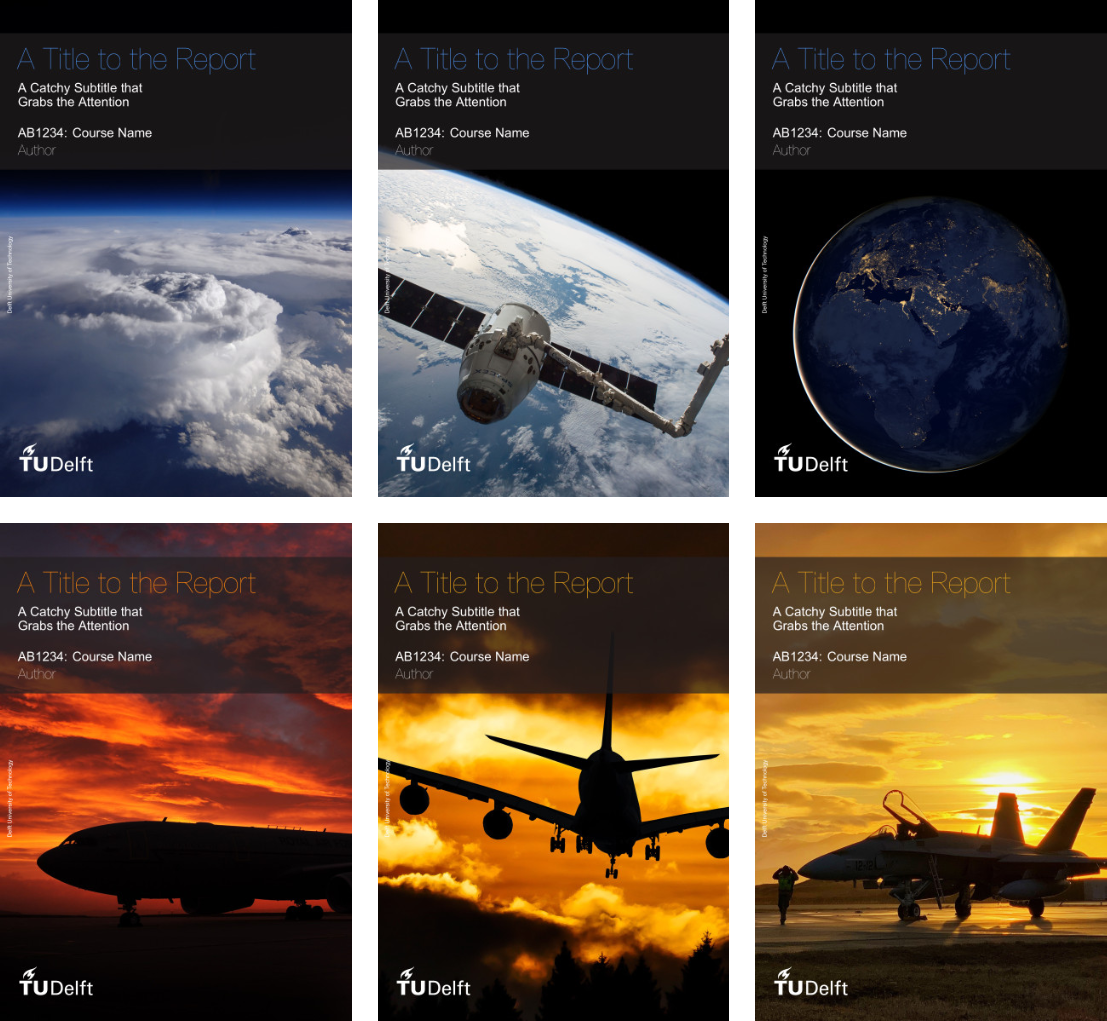
\includegraphics[width=0.75\linewidth]{figures/covers.png}
    \caption{Preview of the included cover images}
\end{figure}

\noindent For the first three images, the title color `4884d6' is recommended. For fourth, the title color `fe860e' is recommended. For the final two, the title color `e3a01b' is recommended. A description with the attribution and license can be found on the next page.

\begin{itemize}
    \item \textbf{cover1.jpg:} Storm Cell Over the Southern Appalachian Mountains by NASA/Stu Broce under CC BY 2.0
    \item \textbf{cover2.jpg:} Canadarm 2 Robotic Arm Grapples SpaceX Dragon by NASA under CC BY-NC 2.0 // Modified
    \item \textbf{cover3.jpg:} City Lights of Africa, Europe, and the Middle East by NASA Earth Observatory under CC BY 2.0
    \item \textbf{cover4.jpg:} Royal Air Force Voyager Transport Tanker Aircraft by Ministry of Defense/Cpl Ashley Keates under OGL v1.0
    \item \textbf{cover5.jpg:} Aircraft Flying in the Sunset by Gerhard Gellinger
    \item \textbf{cover6.jpg:} F18 at Bodo Air Base Norway by Ministerio de Defensa España under CC BY-NC 2.0
\end{itemize}
